\documentclass[a4paper,12pt]{report}
\usepackage[utf8]{inputenc} % To use Unicode (e.g. Turkish) characters
\renewcommand{\labelenumi}{(\roman{enumi})}
\usepackage{amsmath, amsthm, amssymb}
 % Some extra symbols
\usepackage[bottom]{footmisc}
\usepackage{cite}
\usepackage{url}
\usepackage{graphicx}
\usepackage{longtable}

\usepackage{multirow}
\usepackage{subfigure}
\usepackage{algorithm}
\usepackage{algorithmic}
\usepackage{tikz}
\usetikzlibrary{shapes.geometric, arrows, positioning, fit, backgrounds}

\begin{document}

% Title Page
\title{CMPE 492 \\ Project Title}
\author{
Student 1 Enes Sait Besler \\
Student 2 Yusuf Onur Öksüz \\ \\
Advisor: \\ 
H. Birkan Yılmaz
}
\date{}
\maketitle{}
\pagenumbering{roman}
\tableofcontents

\chapter{INTRODUCTION}
\pagenumbering{arabic}

Molecular communication represents a paradigm shift in how we conceptualize information transmission at nanoscale and microscale distances. Unlike traditional electromagnetic wave-based communication systems, molecular communication systems leverage the controlled release, propagation, and detection of molecules to encode and transmit information. This bio-inspired approach opens unprecedented opportunities in domains where conventional wireless communication fails or is impractical, such as intra-body communication networks, environmental monitoring at the microscale, and lab-on-a-chip systems.

However, analyzing and optimizing molecular communication systems presents formidable computational challenges. The physical channel—governed by diffusion processes and Brownian motion—exhibits some Inter-Symbol Interference (ISI) due to the persistent presence of molecules long after their intended transmission interval. Computing exact performance metrics such as bit error rate (BER), channel capacity and information rate requires evaluating conditional probabilities across all possible interference patterns. For a channel with memory length $L$, this translates to $2^L$ distinct cases, rendering brute-force analytical approaches computationally infeasible for realistic scenarios where $L$ can naturally exceed 10-15 symbol durations.

This project addresses this fundamental bottleneck by developing machine learning models capable of accurately estimating communication performance metrics from physical channel parameters without requiring exponential-time calculations. By training deep neural networks on large-scale datasets generated from rigorous physical simulations, we aim to achieve near-instantaneous performance prediction while maintaining high accuracy across diverse channel configurations.

\section{Broad Impact}

The successful development of rapid, accurate performance estimation tools for molecular communication systems has far-reaching implications across multiple domains:

\textbf{Medical Applications:} Molecular communication is a promising technology for intra-body nanonetworks, enabling communication between implanted medical devices, drug delivery systems, and biosensors. Our work facilitates the design and optimization of such networks by allowing researchers and engineers to quickly evaluate performance trade-offs without requiring supercomputing resources. This could accelerate the development of targeted drug delivery systems, real-time health monitoring networks, and coordinated therapeutic interventions at the cellular level.

\textbf{Environmental Monitoring:} Microscale sensor networks deployed in aquatic or terrestrial environments can leverage molecular communication for energy-efficient information exchange. Our estimation framework enables rapid prototyping and performance analysis of such networks for applications including water quality monitoring, pollution detection, and ecosystem health assessment.

\textbf{Synthetic Biology and Bio-computing:} As synthetic biology advances toward engineered cellular communication networks, understanding and optimizing molecular signaling channels becomes crucial. Our AI-driven approach provides a computational foundation for designing bio-compatible communication protocols that can be implemented in living cells or synthetic biological systems.

\textbf{Academic Research Acceleration:} By reducing the computational burden of performance analysis from hours or days to milliseconds, our models democratize access to molecular communication research. Researchers can explore broader parameter spaces, conduct sensitivity analyses, and validate theoretical predictions with unprecedented efficiency, potentially accelerating the pace of discovery in this emerging field.

\textbf{Industrial Design Tools:} The methodologies developed in this project can serve as the foundation for commercial simulation and design tools, similar to how SPICE simulators revolutionized electronic circuit design. Such tools would enable industry adoption of molecular communication technologies in lab-on-a-chip devices, microfluidic systems, and other emerging applications.

\section{Ethical Considerations}

While the technical focus of this project is on computational methods for performance estimation, we recognize several ethical dimensions that warrant consideration:

\textbf{Dual-Use Concerns:} Technologies enabling efficient design of molecular communication systems could potentially be misused for harmful applications, such as covert communication channels or undetectable surveillance systems at microscale. However, the fundamental physical constraints of molecular diffusion (extremely short range, low data rates, high latency) inherently limit such misuse scenarios. Furthermore, our work focuses on performance analysis tools rather than implementation recipes, maintaining a layer of abstraction from direct deployment.

\textbf{Medical Applications Safety:} As this technology may eventually contribute to intra-body nanonetwork designs, rigorous safety validation will be essential. Our performance estimation models must be transparent and verifiable to ensure that predicted behaviors align with actual physical implementations, particularly when human health is at stake. We emphasize the importance of experimental validation and acknowledge that computational predictions, however accurate, cannot substitute for rigorous testing and regulatory approval in medical contexts.

\textbf{Environmental Impact:} The development of AI models requires significant computational resources, contributing to energy consumption and carbon emissions. We mitigate this concern by developing efficient architectures and training procedures that balance accuracy with computational efficiency. Once trained, our models enable rapid inference, potentially reducing the overall computational footprint of molecular communication research by eliminating the need for repeated expensive simulations.

\textbf{Accessibility and Open Science:} We are committed to the principles of open science and plan to make our trained models, datasets (where appropriate), and methodologies publicly available. This ensures that the benefits of our research are accessible to researchers globally, particularly those in resource-constrained institutions who may lack access to high-performance computing infrastructure.

\textbf{Responsible AI Development:} Our models are designed to provide uncertainty estimates and performance metrics that indicate confidence levels. This transparency is crucial for preventing over-reliance on AI predictions and ensuring that human experts maintain oversight in critical applications. We also recognize the importance of testing our models across diverse scenarios to identify and mitigate potential biases or failure modes.

\textbf{Biological System Considerations:} As molecular communication technologies advance toward integration with biological systems, careful consideration of biocompatibility, ecological impact, and unintended consequences becomes paramount. While our work operates primarily in the computational domain, we acknowledge the responsibility to consider downstream implications and to engage with interdisciplinary perspectives spanning biology, medicine, and environmental science.

\chapter{PROJECT DEFINITION AND PLANNING}

\section{Project Definition}

\subsection{Problem Statement}

In Molecular Communication via Diffusion (MCvD) systems, transmitters encode information by releasing molecules into a fluid medium, where they propagate via Brownian motion and are detected by receivers. The fundamental challenge in analyzing such systems lies in the Inter-Symbol Interference (ISI) caused by molecules that remain in the channel beyond their intended symbol duration.

For a channel with memory length $L$, computing the exact channel features such as BER, channel capacity and information rate requires evaluating all $2^L$ possible interference patterns, each with distinct conditional probabilities. This exponential complexity renders traditional analytical approaches infeasible for realistic scenarios where $L \geq 10$. For instance, a modest memory length of $L=14$ requires computing $2^{14} = 16,384$ distinct probability distributions—a task that can take hours or days depending on system parameters.

This computational bottleneck severely limits:
\begin{itemize}
    \item Design space exploration for molecular communication systems
    \item Real-time performance analysis and optimization
    \item Rapid prototyping of communication protocols
    \item Large-scale parameter sensitivity studies
\end{itemize}

\subsection{Project Objectives}

The primary objective of this project is to develop machine learning models that can accurately predict communication performance metrics from physical channel parameters, reducing computation time from hours to milliseconds while maintaining high accuracy.

\textbf{Primary Goals:}
\begin{enumerate}
    \item Develop a physics-based data generation pipeline capable of producing large-scale datasets with theoretical accuracy
    \item Design and implement deep learning architectures tailored to the temporal and statistical characteristics of molecular communication channels
    \item Achieve BER prediction accuracy within 2-3x multiplicative error across BER ranges spanning $10^{-12}$ to $10^{-1}$
    \item Demonstrate inference times under 10 milliseconds per sample on standard hardware
\end{enumerate}

\textbf{Secondary Goals:}
\begin{enumerate}
    \item Investigate model generalization across diverse channel configurations
    \item Develop interpretable feature representations that capture physical channel dynamics
    \item Extend the methodology to information rate and channel capacity estimation (future work)
    \item Create a foundation for AI-driven molecular communication design tools
\end{enumerate}

\subsection{Scope and Delimitations}

\textbf{In Scope:}
\begin{itemize}
    \item On-Off Keying (OOK) modulation scheme
    \item Absorbing spherical receiver model
    \item 3D unbounded diffusion channel
    \item Memory lengths from 3 to 14 symbol durations
    \item Physical parameter ranges: radius (3-7 $\mu$m), distance (3-15 $\mu$m), diffusion coefficient (50-120 $\mu$m$^2$/s), symbol duration (0.5-3 s), molecule count ($10^3$-$10^6$)
    \item BER estimation as the primary performance metric
\end{itemize}

\textbf{Out of Scope:}
\begin{itemize}
    \item Alternative modulation schemes (CSK, MoSK, etc.)
    \item Non-spherical receiver geometries
    \item Flow-assisted or bounded channel environments
    \item Real-time physical implementation or hardware design
    \item Experimental validation with actual molecular systems
\end{itemize}

\section{Project Planning}

\subsection{Project Time and Resource Estimation}

The project spans one semester (Spring 2026, 13 weeks total) with the following phase breakdown:

\textbf{Phase 1: BER Estimation (Weeks 1-7)}
\begin{itemize}
    \item Literature review on molecular communication and ML for physical systems
    \item Implementation of physical channel simulation (hitting probability calculations)
    \item Development of vectorized BER computation with Gaussian approximation
    \item Large-scale dataset generation (achieved: 5,000,000+ samples)
    \item Baseline CNN model development and training
    \item Design and implementation of multi-scale residual architecture (BERMultiScaleResCNNv2)
    \item Integration of advanced components (self-attention, FiLM layers, SE blocks)
    \item Development of stable multi-objective loss function
    \item Model evaluation and validation across BER regimes
\end{itemize}

\textbf{Phase 2: Information Rate Estimation (Weeks 8-13)}
\begin{itemize}
    \item Extension of physical simulation to compute mutual information and channel capacity
    \item Development of information rate calculation algorithms for molecular channels
    \item Dataset generation for information rate prediction (target: 1,000,000+ samples)
    \item Adaptation of neural network architecture for information rate estimation
    \item Model training and hyperparameter optimization
    \item Comprehensive evaluation and comparison with analytical bounds
    \item Documentation, visualization, and final report preparation
\end{itemize}

\textbf{Resource Requirements:}
\begin{itemize}
    \item \textbf{Computational:} GPU-enabled workstation for model training (NVIDIA RTX 3080 or equivalent); estimated 100-200 GPU-hours for full training pipeline
    \item \textbf{Storage:} Approximately 5-10 GB for datasets and trained models
    \item \textbf{Software:} Python 3.8+, PyTorch, NumPy, SciPy, Pandas, scikit-learn (all open-source)
    \item \textbf{Human Resources:} Two team members with complementary skills in ML/DL and communication theory
\end{itemize}

\subsection{Success Criteria}

\textbf{Phase 1 (BER Estimation) - COMPLETED:}
\begin{itemize}
    \item Model achieves MAE $< 0.5$ in log$_{10}$(BER) space (approximately 3x multiplicative error)
    \item Inference time at least 1000x faster than analytical computation ($<$ 10ms vs. $>$ 10 seconds)
    \item Reliable predictions across at least 6 orders of magnitude in BER ($10^{-9}$ to $10^{-3}$)
    \item Dataset generation and validation exceeding 1,000,000 samples
\end{itemize}

\textbf{Phase 2 (Information Rate Estimation) - IN PROGRESS:}
\begin{itemize}
    \item Model predicts information rate with relative error $< 15\%$ on held-out test data
    \item Successful implementation of mutual information calculation algorithms
    \item Model generalizes across diverse channel memory lengths and parameter configurations
    \item Comprehensive evaluation against theoretical Shannon capacity bounds
\end{itemize}

\subsection{Risk Analysis}

\textbf{Risk 1: Data Quality and Validity}
\begin{itemize}
    \item \textbf{Description:} Errors in physical simulation or approximation methods could propagate to training data, causing models to learn incorrect relationships
    \item \textbf{Likelihood:} Medium
    \item \textbf{Impact:} High
    \item \textbf{Mitigation:} Rigorous validation against published analytical results for small memory lengths; cross-validation with Monte Carlo simulations; peer review of mathematical formulations
\end{itemize}

\textbf{Risk 2: Model Overfitting or Poor Generalization}
\begin{itemize}
    \item \textbf{Description:} Model may memorize training distribution patterns rather than learning underlying physical relationships
    \item \textbf{Likelihood:} Medium
    \item \textbf{Impact:} High
    \item \textbf{Mitigation:} Stratified train/validation/test splits; augmentation with synthetic random samples; regularization techniques (dropout, weight decay); testing on extrapolation scenarios
\end{itemize}

\textbf{Risk 3: Computational Resource Constraints}
\begin{itemize}
    \item \textbf{Description:} Insufficient GPU resources or training time may limit model complexity or dataset size
    \item \textbf{Likelihood:} Low-Medium
    \item \textbf{Impact:} Medium
    \item \textbf{Mitigation:} Efficient data generation pipeline with incremental saving; distributed training capabilities; access to university computing clusters if needed; focus on architectural efficiency
\end{itemize}

\textbf{Risk 4: Loss Function Instability}
\begin{itemize}
    \item \textbf{Description:} Predicting values across 12 orders of magnitude may cause numerical instability, NaN losses, or gradient explosion
    \item \textbf{Likelihood:} High (already encountered and addressed)
    \item \textbf{Impact:} High
    \item \textbf{Mitigation:} Log-scale predictions; stable loss formulations with clamping; gradient clipping; extensive numerical stability testing; non-finite value detection during training
\end{itemize}

\textbf{Risk 5: Time Management and Scope Creep}
\begin{itemize}
    \item \textbf{Description:} Ambitious goals may lead to incomplete implementation or rushed evaluation
    \item \textbf{Likelihood:} Medium
    \item \textbf{Impact:} Medium
    \item \textbf{Mitigation:} Phased development with clear milestones; prioritization of core functionality over extensions; regular progress reviews with advisor; documented decision points for scope adjustment
\end{itemize}

\subsection{Team Work}

This project is a collaborative effort between two team members with complementary expertise:

\textbf{Enes Sait Besler:}
\begin{itemize}
    \item Primary responsibilities: Deep learning architecture design, model implementation
    \item Secondary responsibilities: Data preprocessing, performance evaluation, documentation
\end{itemize}

\textbf{Yusuf Onur Öksüz:}
\begin{itemize}
    \item Primary responsibilities: Physical channel modeling, mathematical formulation, data generation pipeline
    \item Secondary responsibilities: Validation against analytical methods,  visualization
\end{itemize}

\textbf{Collaboration Framework:}
\begin{itemize}
    \item Weekly team meetings to synchronize progress and resolve blockers
    \item Bi-weekly advisor meetings for technical guidance and milestone reviews
    \item Git-based version control with feature branching for parallel development
    \item Shared documentation in project wiki for knowledge transfer
    \item Code review process for critical components (simulation, model architecture, loss functions)
\end{itemize}

\textbf{Communication Channels:}
\begin{itemize}
    \item GitHub repository for code and issue tracking
    \item Shared LaTeX document for report writing
    \item Instant messaging for quick coordination
    \item Scheduled video calls for in-depth technical discussions
\end{itemize}

\chapter{RELATED WORK}
Literature survey.

\chapter{METHODOLOGY}

Our methodology consists of four main components: physical channel modeling, data generation, neural network architecture design, and training procedures.

\section{Physical Channel Model}

We consider a point transmitter at distance $d$ from a spherical absorbing receiver of radius $r_{rx}$. The transmitter uses On-Off Keying (OOK) modulation, transmitting $N$ molecules for bit '1' and zero for bit '0' with symbol duration $T_s$. Molecules propagate via Brownian motion with diffusion coefficient $D$.

The cumulative hitting probability is:
\begin{equation}
F_{hit}(t) = \frac{r_{rx}}{r_{rx} + d} \cdot \text{erfc}\left(\frac{d}{\sqrt{4Dt}}\right)
\end{equation}

The interval hitting probability for the $i$-th symbol is:
\begin{equation}
P[i] = F_{hit}((i+1)T_s) - F_{hit}(iT_s)
\end{equation}

Channel memory length $L$ is determined adaptively by accumulating hitting probabilities until reaching 70\% of the asymptotic probability $f_{\infty} = r_{rx}/(r_{rx} + d)$.

\section{BER Calculation}

For a binary sequence $(b_0, b_1, \ldots, b_{L-1})$, the expected arrival count and variance are:
\begin{equation}
\mu = N \sum_{i=0}^{L-1} b_i \cdot P[i], \quad \sigma^2 = N \sum_{i=0}^{L-1} b_i \cdot P[i] \cdot (1 - P[i])
\end{equation}

Using Gaussian approximation for large $N$, the conditional bit error probability with threshold $\tau$ is:
\begin{equation}
P_e | b_0 =
\begin{cases}
Q\left(\frac{\mu - \tau}{\sigma}\right) & \text{if } b_0 = 1 \\
Q\left(\frac{\tau - \mu}{\sigma}\right) & \text{if } b_0 = 0
\end{cases}
\end{equation}

The overall BER requires averaging over all $2^L$ sequences, which becomes infeasible for $L \geq 10$.

\section{Data Generation Pipeline}

\subsection{Physics-Based Samples}

Physical parameters are randomly sampled: $r_{rx} \in [3, 7]$ $\mu$m, $d \in [3, 15]$ $\mu$m, $D \in [50, 120]$ $\mu$m$^2$/s, $T_s \in [0.5, 3.0]$ s, $N \in [10^3, 10^6]$ (log-uniform). For each sample, we compute memory length $L$ (up to 14), hitting probabilities, select threshold $\tau$, and calculate BER via vectorized evaluation of all $2^L$ sequences.

\subsection{Synthetic Samples}

To improve robustness, we generate synthetic samples with random monotonically decreasing probability sequences, avoiding overfitting to specific physical patterns.

\subsection{Preprocessing}

Features are log-transformed and standardized. Input consists of 6 channels: scaled means, log-variances, normalized position, absolute values, SNR proxy, and first-position indicator. Data is split 70\%/15\%/15\% (train/val/test) with stratification on log(BER).

\section{Neural Network Architecture}

We developed BERMultiScaleResCNNv2, combining:
\begin{itemize}
    \item Dual-stem 1D CNN encoders for mean and variance channels
    \item Multi-scale residual blocks (parallel branches with kernel sizes 3, 5, and dilated 3)
    \item Squeeze-and-Excitation attention for channel recalibration
    \item Threshold-conditioned FiLM layers
    \item Learned positional embeddings
    \item Multi-head self-attention for long-range dependencies
    \item Hierarchical multi-stage pooling
    \item MLP prediction head outputting log$_{10}$(BER)
\end{itemize}

The architecture processes 6-channel sequences (length up to 14) through three progressive stages (32→64→96→128 channels) with downsampling and attention mechanisms.

\section{Training Procedure}

We employ a stable multi-objective loss combining log-scale and raw-scale Huber losses:
\begin{equation}
\mathcal{L} = 0.9 \cdot \mathcal{L}_{\text{Huber}}^{\log}(y_{\log}, \hat{y}_{\log}) + 0.1 \cdot \mathcal{L}_{\text{Huber}}^{\text{raw}}(10^{y_{\log}}, 10^{\hat{y}_{\log}})
\end{equation}

Predictions are clamped to $[-12, 0]$ before exponentiation to prevent overflow.

\textbf{Optimization:} AdamW optimizer with learning rate $10^{-4}$, batch size 256, gradient clipping (max norm 1.0), ReduceLROnPlateau scheduler, and early stopping (patience 12 epochs).

\textbf{Stability:} Non-finite value detection, gradient monitoring, prediction clamping, and epsilon terms in log transformations.

\textbf{Evaluation Metrics:} Log-scale MAE/RMSE, multiplicative error factor ($10^{\text{RMSE}_{\log}}$), raw-scale MAE/RMSE, and per-regime metrics (low/mid/high BER).

\chapter{REQUIREMENTS SPECIFICATION}

\section{Functional Requirements}

\subsection{Data Generation Module}
\begin{itemize}
    \item \textbf{FR1:} Generate physics-based samples from molecular communication channel parameters
    \item \textbf{FR2:} Generate synthetic samples with random probability sequences
    \item \textbf{FR3:} Compute hitting probabilities using analytical formulas (erfc-based)
    \item \textbf{FR4:} Calculate BER via vectorized evaluation of all $2^L$ sequences
    \item \textbf{FR5:} Adaptively determine channel memory length $L$ based on coverage threshold
    \item \textbf{FR6:} Save generated data incrementally to prevent loss during long generation runs
\end{itemize}

\subsection{Data Processing Module}
\begin{itemize}
    \item \textbf{FR7:} Load and validate CSV datasets
    \item \textbf{FR8:} Apply log transformations to handle wide dynamic ranges
    \item \textbf{FR9:} Construct 6-channel feature sequences from raw data
    \item \textbf{FR10:} Standardize features using fitted scalers
    \item \textbf{FR11:} Split data with stratification on BER values
    \item \textbf{FR12:} Save and load scalers for consistent preprocessing
\end{itemize}

\subsection{Model Training Module}
\begin{itemize}
    \item \textbf{FR13:} Initialize neural network architecture with configurable hyperparameters
    \item \textbf{FR14:} Train model using multi-objective loss function
    \item \textbf{FR15:} Monitor training/validation loss and metrics per epoch
    \item \textbf{FR16:} Implement early stopping based on validation performance
    \item \textbf{FR17:} Save best model checkpoint during training
    \item \textbf{FR18:} Detect and handle numerical instabilities (NaN/Inf values)
\end{itemize}

\subsection{Model Evaluation Module}
\begin{itemize}
    \item \textbf{FR19:} Evaluate model on held-out test data
    \item \textbf{FR20:} Compute multiple performance metrics (MAE, RMSE, multiplicative error)
    \item \textbf{FR21:} Generate per-regime evaluation (low/mid/high BER)
    \item \textbf{FR22:} Compare predictions with ground truth across BER ranges
\end{itemize}

\subsection{Inference Module}
\begin{itemize}
    \item \textbf{FR23:} Load trained model and scalers
    \item \textbf{FR24:} Accept new channel parameters as input
    \item \textbf{FR25:} Predict BER/information rate in real-time ($< 10$ms per sample)
    \item \textbf{FR26:} Return predictions with confidence estimates
\end{itemize}

\section{Non-Functional Requirements}

\subsection{Performance Requirements}
\begin{itemize}
    \item \textbf{NFR1:} Model inference time must be at least 1000x faster than analytical computation
    \item \textbf{NFR2:} Data generation should process at least 100 samples per second
    \item \textbf{NFR3:} Model training should converge within 100 epochs
    \item \textbf{NFR4:} System should handle datasets up to 5 million samples
\end{itemize}

\subsection{Accuracy Requirements}
\begin{itemize}
    \item \textbf{NFR5:} Model MAE in log$_{10}$(BER) space must be $< 0.5$
    \item \textbf{NFR6:} Model should maintain accuracy across 6+ orders of magnitude
    \item \textbf{NFR7:} Predictions should remain stable for all valid parameter ranges
\end{itemize}

\subsection{Usability Requirements}
\begin{itemize}
    \item \textbf{NFR8:} Code should be modular and well-documented
    \item \textbf{NFR9:} Training pipeline should be reproducible with fixed random seeds
    \item \textbf{NFR10:} Scripts should provide clear progress logging and error messages
\end{itemize}

\subsection{Reliability Requirements}
\begin{itemize}
    \item \textbf{NFR11:} Data generation should save incrementally to prevent loss on interruption
    \item \textbf{NFR12:} Training should detect and halt on numerical instabilities
    \item \textbf{NFR13:} Model checkpoints should be saved periodically
\end{itemize}

\section{System Constraints}

\begin{itemize}
    \item \textbf{C1:} System requires GPU for efficient model training
    \item \textbf{C2:} Maximum channel memory length limited to $L = 14$ for computational feasibility
    \item \textbf{C3:} BER calculation uses Gaussian approximation, valid for $N \geq 1000$
    \item \textbf{C4:} System operates on pre-generated datasets, not real-time physical experiments
\end{itemize}

\chapter{DESIGN}

\section{Information Structure}

The system's information structure consists of six primary entities representing the data flow from physical parameters to trained models.

\subsection{Data Entities}

\textbf{Physical Channel Parameters:}
Input parameters defining the molecular communication channel: receiver radius ($r_{rx}$), transmitter-receiver distance ($d$), diffusion coefficient ($D$), symbol duration ($T_s$), and molecule count ($N$).

\textbf{Channel Response:}
Derived characteristics including memory length ($L$), hitting probability sequence ($P[0..L-1]$), variance sequence, and detection threshold ($\tau$). Computed from physical parameters via analytical formulas.

\textbf{Training Sample:}
Individual data point containing sample ID, type (physics-based or synthetic), and ground truth BER value. Generated by exhaustive evaluation of $2^L$ interference patterns.

\textbf{Feature Sequence:}
Preprocessed 6-channel tensor representation: scaled means, log-variances, position encoding, absolute values, SNR proxy, and first-position indicator. Each sequence has variable length (3-14 time steps).

\textbf{Model Checkpoint:}
Persistent storage of trained model including architecture name, timestamp, state dictionary (neural network weights), and validation loss. Enables model reloading for inference.

\textbf{Scaler Objects:}
Fitted StandardScaler instances for each feature channel, ensuring consistent normalization between training and inference phases.

\subsection{Entity Relationships}

\begin{itemize}
    \item Physical Parameters $\rightarrow$ Channel Response (1:1, via analytical computation)
    \item Channel Response $\rightarrow$ Training Sample (1:1, via BER calculation)
    \item Training Sample $\rightarrow$ Feature Sequence (1:1, via preprocessing)
    \item Feature Sequences $\rightarrow$ Model Checkpoint (N:1, via training)
    \item Feature Sequences $\leftrightarrow$ Scaler Objects (N:1, for normalization)
\end{itemize}

\subsection{Entity-Relationship Diagram}

\begin{figure}[h!]
\centering
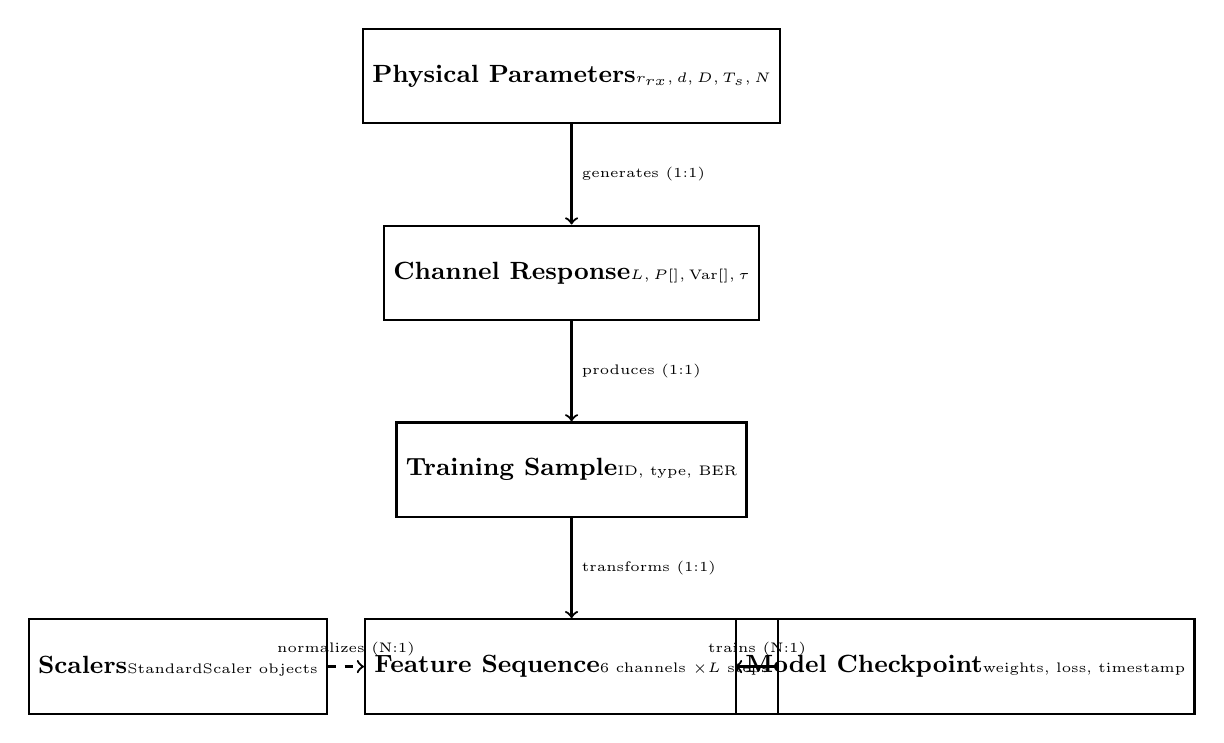
\begin{tikzpicture}[
    entity/.style={rectangle, draw, thick, minimum width=3cm, minimum height=1.2cm, text centered, font=\small},
    relation/.style={diamond, draw, thick, aspect=2, minimum width=1.5cm, minimum height=0.8cm, text centered, font=\tiny},
    arrow/.style={->, thick}
]
    % Entities
    \node[entity] (params) {\textbf{Physical Parameters}\\{\tiny $r_{rx}, d, D, T_s, N$}};
    \node[entity, below of=params, yshift=-1.5cm] (response) {\textbf{Channel Response}\\{\tiny $L, P[], \text{Var}[], \tau$}};
    \node[entity, below of=response, yshift=-1.5cm] (sample) {\textbf{Training Sample}\\{\tiny ID, type, BER}};
    \node[entity, below of=sample, yshift=-1.5cm] (features) {\textbf{Feature Sequence}\\{\tiny 6 channels $\times L$ steps}};
    \node[entity, right of=features, xshift=4cm] (model) {\textbf{Model Checkpoint}\\{\tiny weights, loss, timestamp}};
    \node[entity, left of=features, xshift=-4cm] (scalers) {\textbf{Scalers}\\{\tiny StandardScaler objects}};

    % Relations
    \draw[arrow] (params) -- node[right, font=\tiny] {generates (1:1)} (response);
    \draw[arrow] (response) -- node[right, font=\tiny] {produces (1:1)} (sample);
    \draw[arrow] (sample) -- node[right, font=\tiny] {transforms (1:1)} (features);
    \draw[arrow] (features) -- node[above, font=\tiny] {trains (N:1)} (model);
    \draw[arrow, dashed] (scalers) -- node[above, font=\tiny] {normalizes (N:1)} (features);
\end{tikzpicture}
\caption{Entity-relationship diagram showing data structure}
\label{fig:er-diagram}
\end{figure}

\section{Information Flow}

The system's information flow spans three primary processes: data generation, model training, and inference.

\subsection{Data Generation Workflow}

The data generation process operates continuously:
\begin{enumerate}
    \item Sample physical parameters from uniform distributions
    \item Compute hitting probabilities $P[i]$ using erfc-based formulas
    \item Determine adaptive memory length $L$ (70\% coverage threshold)
    \item Select detection threshold $\tau$ from realistic range
    \item Generate all $2^L$ binary sequences
    \item Calculate BER via Gaussian approximation for each sequence
    \item Average BER across sequences to obtain final label
    \item Buffer samples and save incrementally to CSV (100-row batches)
    \item Repeat until user interruption
\end{enumerate}

\subsection{Model Training Workflow}

Training follows a supervised learning pipeline:
\begin{enumerate}
    \item Load CSV dataset and validate required columns
    \item Apply log transformations (BER, threshold, variances, N)
    \item Engineer 6-channel feature sequences from raw data
    \item Fit StandardScalers on training split
    \item Stratified splitting (70\%/15\%/15\% train/val/test)
    \item Initialize BERMultiScaleResCNNv2 architecture
    \item \textbf{Training loop per epoch:}
    \begin{itemize}
        \item Forward pass on mini-batches
        \item Compute multi-objective loss
        \item Backward pass and gradient clipping
        \item Check for NaN/Inf (halt if detected)
        \item Validate on validation set
        \item Update learning rate via scheduler
        \item Save checkpoint if best validation loss
        \item Check early stopping criterion
    \end{itemize}
    \item Evaluate final model on test set
    \item Save best model checkpoint and scalers
\end{enumerate}

\subsection{Inference Workflow}

Prediction for new channel parameters:
\begin{enumerate}
    \item Load trained model checkpoint and scaler objects
    \item Accept physical parameters ($r_{rx}$, $d$, $D$, $T_s$, $N$, $\tau$)
    \item Compute hitting probabilities and variances
    \item Construct 6-channel feature sequence
    \item Apply standardization using loaded scalers
    \item Forward pass through model
    \item Obtain log$_{10}$(BER) prediction
    \item Convert to raw BER: $\text{BER} = 10^{\text{prediction}}$
    \item Return prediction (typically $< 10$ms)
\end{enumerate}

\subsection{Process Interactions}

Key interactions between components:
\begin{itemize}
    \item \textbf{DataLoader $\leftrightarrow$ Preprocessor:} Raw samples transformed to normalized features
    \item \textbf{Model $\leftrightarrow$ Optimizer:} Iterative weight updates via backpropagation
    \item \textbf{Model $\leftrightarrow$ Storage:} Periodic checkpoint saving during training
    \item \textbf{Scalers $\leftrightarrow$ Features:} Bidirectional dependency for consistent normalization
\end{itemize}

\subsection{System Diagrams}

\subsubsection{Complete Pipeline Overview}

\begin{figure}[h!]
\centering
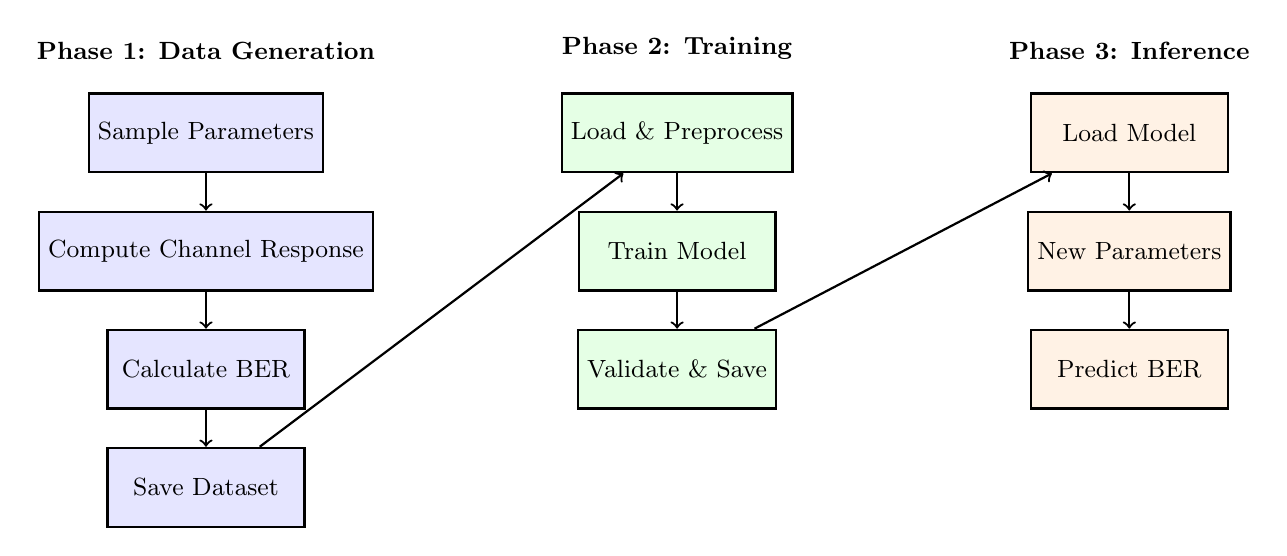
\begin{tikzpicture}[
    node distance=1.5cm,
    box/.style={rectangle, draw, thick, minimum width=2.5cm, minimum height=1cm, text centered, font=\small},
    arrow/.style={->, thick}
]
    % Phase 1
    \node[box, fill=blue!10] (params) {Sample Parameters};
    \node[box, fill=blue!10, below of=params] (response) {Compute Channel Response};
    \node[box, fill=blue!10, below of=response] (ber) {Calculate BER};
    \node[box, fill=blue!10, below of=ber] (save) {Save Dataset};

    % Phase 2
    \node[box, fill=green!10, right=3cm of params] (load) {Load \& Preprocess};
    \node[box, fill=green!10, below of=load] (train) {Train Model};
    \node[box, fill=green!10, below of=train] (validate) {Validate \& Save};

    % Phase 3
    \node[box, fill=orange!10, right=3cm of load] (loadmodel) {Load Model};
    \node[box, fill=orange!10, below of=loadmodel] (newparams) {New Parameters};
    \node[box, fill=orange!10, below of=newparams] (predict) {Predict BER};

    % Arrows
    \draw[arrow] (params) -- (response);
    \draw[arrow] (response) -- (ber);
    \draw[arrow] (ber) -- (save);
    \draw[arrow] (save) -- (load);
    \draw[arrow] (load) -- (train);
    \draw[arrow] (train) -- (validate);
    \draw[arrow] (validate) -- (loadmodel);
    \draw[arrow] (loadmodel) -- (newparams);
    \draw[arrow] (newparams) -- (predict);

    % Phase labels
    \node[above=0.3cm of params, font=\small\bfseries] {Phase 1: Data Generation};
    \node[above=0.3cm of load, font=\small\bfseries] {Phase 2: Training};
    \node[above=0.3cm of loadmodel, font=\small\bfseries] {Phase 3: Inference};
\end{tikzpicture}
\caption{Complete system pipeline from data generation to inference}
\label{fig:pipeline}
\end{figure}

\subsubsection{Data Flow Diagram}

\begin{figure}[h!]
\centering
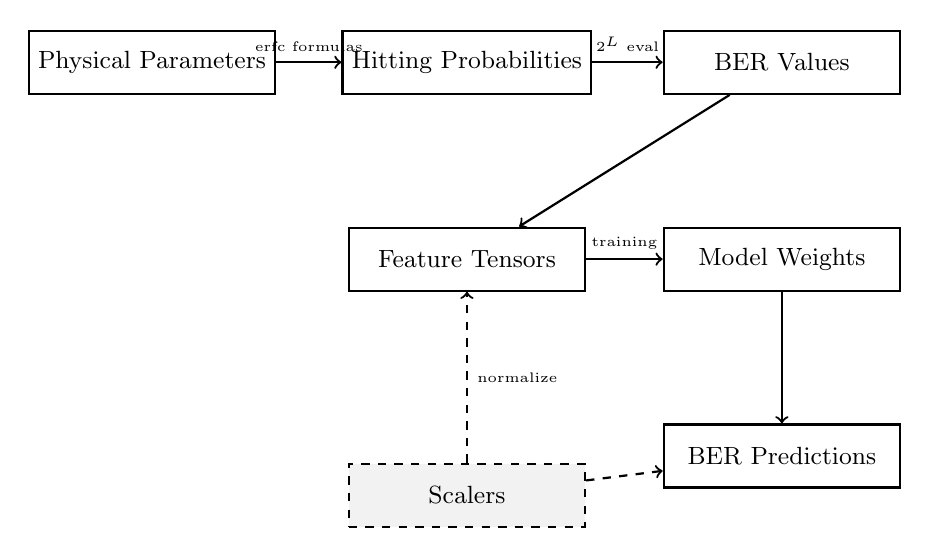
\begin{tikzpicture}[
    node distance=2cm,
    process/.style={rectangle, draw, thick, minimum width=3cm, minimum height=0.8cm, text centered, font=\small},
    arrow/.style={->, thick}
]
    \node[process] (params) {Physical Parameters};
    \node[process, right of=params, xshift=2cm] (hitting) {Hitting Probabilities};
    \node[process, right of=hitting, xshift=2cm] (ber) {BER Values};
    \node[process, below of=hitting, yshift=-0.5cm] (features) {Feature Tensors};
    \node[process, right of=features, xshift=2cm] (model) {Model Weights};
    \node[process, below of=model, yshift=-0.5cm] (pred) {BER Predictions};

    \node[process, dashed, below of=features, yshift=-1cm, fill=gray!10] (scalers) {Scalers};

    \draw[arrow] (params) -- node[above, font=\tiny] {erfc formulas} (hitting);
    \draw[arrow] (hitting) -- node[above, font=\tiny] {$2^L$ eval} (ber);
    \draw[arrow] (ber) -- (features);
    \draw[arrow] (features) -- node[above, font=\tiny] {training} (model);
    \draw[arrow] (model) -- (pred);
    \draw[arrow, dashed] (scalers) -- node[right, font=\tiny] {normalize} (features);
    \draw[arrow, dashed] (scalers) -- (pred);
\end{tikzpicture}
\caption{Data flow from physical parameters to BER predictions}
\label{fig:dataflow}
\end{figure}

\subsubsection{Training Loop Activity Diagram}

\begin{figure}[h!]
\centering
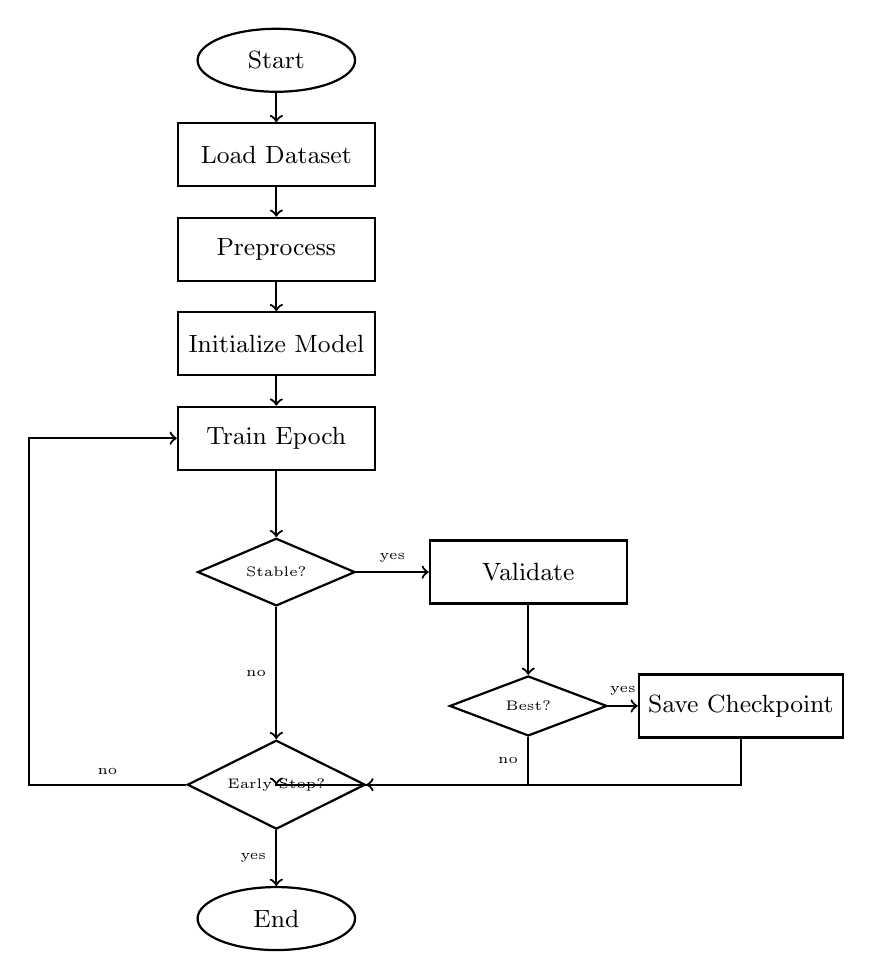
\begin{tikzpicture}[
    node distance=1.2cm,
    startstop/.style={ellipse, draw, thick, minimum width=2cm, minimum height=0.8cm, text centered, font=\small},
    process/.style={rectangle, draw, thick, minimum width=2.5cm, minimum height=0.8cm, text centered, font=\small},
    decision/.style={diamond, draw, thick, aspect=2, minimum width=2cm, text centered, font=\tiny},
    arrow/.style={->, thick}
]
    \node[startstop] (start) {Start};
    \node[process, below of=start] (load) {Load Dataset};
    \node[process, below of=load] (preprocess) {Preprocess};
    \node[process, below of=preprocess] (init) {Initialize Model};
    \node[process, below of=init] (epoch) {Train Epoch};
    \node[decision, below of=epoch, yshift=-0.5cm] (stable) {Stable?};
    \node[process, right of=stable, xshift=2cm] (validate) {Validate};
    \node[decision, below of=validate, yshift=-0.5cm] (best) {Best?};
    \node[process, right of=best, xshift=1.5cm] (save) {Save Checkpoint};
    \node[decision, below of=stable, yshift=-1.5cm] (early) {Early Stop?};
    \node[startstop, below of=early, yshift=-0.5cm] (end) {End};

    \draw[arrow] (start) -- (load);
    \draw[arrow] (load) -- (preprocess);
    \draw[arrow] (preprocess) -- (init);
    \draw[arrow] (init) -- (epoch);
    \draw[arrow] (epoch) -- (stable);
    \draw[arrow] (stable) -- node[above, font=\tiny] {yes} (validate);
    \draw[arrow] (stable) -- node[left, font=\tiny] {no} (early);
    \draw[arrow] (validate) -- (best);
    \draw[arrow] (best) -- node[above, font=\tiny] {yes} (save);
    \draw[arrow] (best) -- node[left, font=\tiny] {no} ++(0,-1) -| (early);
    \draw[arrow] (save) |- (early);
    \draw[arrow] (early) -- node[left, font=\tiny] {yes} (end);
    \draw[arrow] (early.west) -- node[above, font=\tiny] {no} ++(-2,0) |- (epoch);
\end{tikzpicture}
\caption{Training loop with stability checks and early stopping}
\label{fig:training}
\end{figure}

\section{System Design}

\subsection{Module Architecture}

The system consists of three primary modules with clear separation of concerns.

\begin{figure}[h!]
\centering
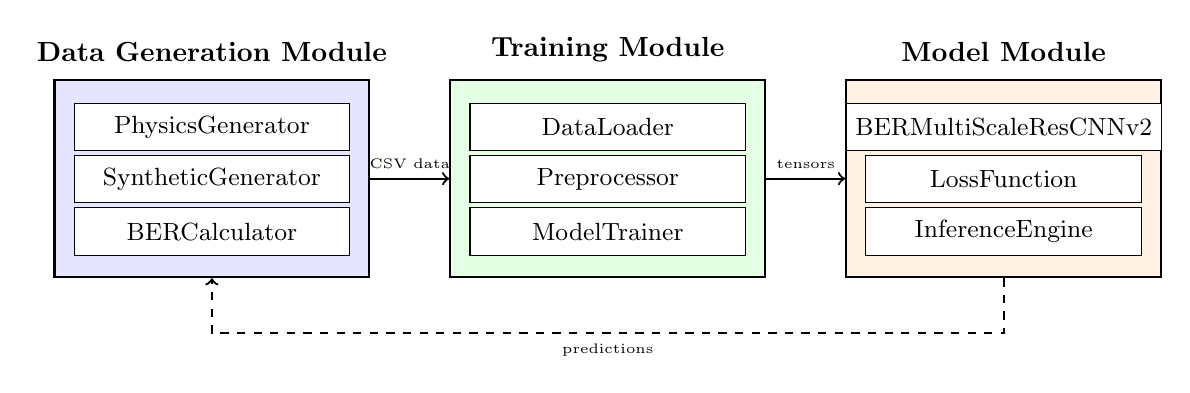
\begin{tikzpicture}[
    module/.style={rectangle, draw, thick, minimum width=4cm, minimum height=2.5cm, text centered},
    component/.style={rectangle, draw, minimum width=3.5cm, minimum height=0.6cm, text centered, font=\small},
    arrow/.style={->, thick}
]
    % Modules
    \node[module, fill=blue!10] (datagen) at (0,0) {};
    \node[above=0.1cm of datagen.north, font=\bfseries] {Data Generation Module};
    \node[component, fill=white, below=0.3cm of datagen.north] (gen1) {PhysicsGenerator};
    \node[component, fill=white, below=0.05cm of gen1] (gen2) {SyntheticGenerator};
    \node[component, fill=white, below=0.05cm of gen2] (gen3) {BERCalculator};

    \node[module, fill=green!10, right=1cm of datagen] (training) {};
    \node[above=0.1cm of training.north, font=\bfseries] {Training Module};
    \node[component, fill=white, below=0.3cm of training.north] (tr1) {DataLoader};
    \node[component, fill=white, below=0.05cm of tr1] (tr2) {Preprocessor};
    \node[component, fill=white, below=0.05cm of tr2] (tr3) {ModelTrainer};

    \node[module, fill=orange!10, right=1cm of training] (model) {};
    \node[above=0.1cm of model.north, font=\bfseries] {Model Module};
    \node[component, fill=white, below=0.3cm of model.north] (m1) {BERMultiScaleResCNNv2};
    \node[component, fill=white, below=0.05cm of m1] (m2) {LossFunction};
    \node[component, fill=white, below=0.05cm of m2] (m3) {InferenceEngine};

    % Arrows
    \draw[arrow] (datagen.east) -- node[above, font=\tiny] {CSV data} (training.west);
    \draw[arrow] (training.east) -- node[above, font=\tiny] {tensors} (model.west);
    \draw[arrow, dashed] (model.south) -- ++(0,-0.7) -| node[below, font=\tiny, pos=0.25] {predictions} (datagen.south);
\end{tikzpicture}
\caption{High-level module architecture}
\label{fig:modules}
\end{figure}

\subsection{Class Diagram}

Key classes and their relationships:

\begin{figure}[h!]
\centering
\begin{tikzpicture}[
    class/.style={rectangle, draw, thick, minimum width=3.2cm, text centered, font=\small},
    arrow/.style={->, thick},
    inherit/.style={->, thick, -triangle 45},
    compose/.style={->, thick, -diamond}
]
    % Main classes
    \node[class] (dataset) at (0,0) {
        \textbf{TensorDataset}\\
        \rule{3cm}{0.4pt}\\
        sequences\\
        thresholds\\
        labels\\
        \rule{3cm}{0.4pt}\\
        \_\_getitem\_\_()\\
        \_\_len\_\_()
    };

    \node[class, right=2cm of dataset] (model) {
        \textbf{BERMultiScaleResCNNv2}\\
        \rule{3cm}{0.4pt}\\
        stem\_encoders\\
        residual\_blocks\\
        attention\_layers\\
        \rule{3cm}{0.4pt}\\
        forward()\\
        predict()
    };

    \node[class, below=1.5cm of dataset] (scaler) {
        \textbf{StandardScaler}\\
        \rule{3cm}{0.4pt}\\
        mean\_\\
        scale\_\\
        \rule{3cm}{0.4pt}\\
        fit()\\
        transform()
    };

    \node[class, below=1.5cm of model] (loss) {
        \textbf{MultiObjectiveLoss}\\
        \rule{3cm}{0.4pt}\\
        alpha\\
        beta\\
        \rule{3cm}{0.4pt}\\
        forward()\\
        huber()
    };

    \node[class, right=2cm of model] (trainer) {
        \textbf{ModelTrainer}\\
        \rule{3cm}{0.4pt}\\
        model\\
        optimizer\\
        criterion\\
        \rule{3cm}{0.4pt}\\
        train\_epoch()\\
        validate()\\
        save\_checkpoint()
    };

    % Relationships
    \draw[compose] (trainer.west) -- node[above, font=\tiny] {uses} (model.east);
    \draw[compose] (trainer.south) -- ++(0,-0.5) -| node[below, font=\tiny, pos=0.25] {uses} (loss.east);
    \draw[arrow] (dataset.east) -- node[above, font=\tiny] {feeds} (model.west);
    \draw[arrow] (scaler.north) -- node[left, font=\tiny] {normalizes} (dataset.south);
\end{tikzpicture}
\caption{Core class relationships}
\label{fig:classes}
\end{figure}

\subsection{Component Breakdown}

\textbf{Data Generation Module:}
\begin{itemize}
    \item \texttt{data\_generation.py}: Main script implementing physics-based and synthetic sample generation
    \item Functions: \texttt{Fhit\_function()}, \texttt{calculate\_ber\_vectorized()}, \texttt{generate\_physics\_sample()}
\end{itemize}

\textbf{Training Module:}
\begin{itemize}
    \item \texttt{train.py}: Complete training pipeline with preprocessing and evaluation
    \item Functions: \texttt{prepare\_data()}, \texttt{train\_engine()}, \texttt{evaluate()}
\end{itemize}

\textbf{Model Architecture:}
\begin{itemize}
    \item Classes: \texttt{BERMultiScaleResCNNv2}, \texttt{MultiScaleResidualBlock}, \texttt{SqueezeExcite1D}
    \item \texttt{ThresholdFiLM}, \texttt{LightSelfAttention1D}, \texttt{StableMultiObjectiveBERLoss}
\end{itemize}

\subsection{Data Flow Between Components}

\begin{enumerate}
    \item \textbf{DataGenerator} produces CSV files
    \item \textbf{DataLoader} reads and validates CSV data
    \item \textbf{Preprocessor} applies transformations and creates feature tensors
    \item \textbf{TensorDataset} wraps tensors for batch iteration
    \item \textbf{Model} processes batches and produces predictions
    \item \textbf{LossFunction} computes training objective
    \item \textbf{Optimizer} updates model weights
    \item \textbf{ModelTrainer} orchestrates the entire training loop
    \item \textbf{InferenceEngine} loads checkpoints for prediction
\end{enumerate}

\section{User Interface Design (if applicable)}

\chapter{IMPLEMENTATION AND TESTING}

\section{Implementation}

\subsection{Development Environment}

The project is implemented in Python 3.8+ using PyTorch for deep learning, NumPy/SciPy for numerical computations, and Pandas/scikit-learn for data processing. Development follows a modular structure with three main scripts:

\begin{itemize}
    \item \textbf{data\_generation.py}: Physics-based and synthetic sample generation with vectorized BER computation
    \item \textbf{train.py}: Advanced model training pipeline with BERMultiScaleResCNNv2 architecture
    \item \textbf{train\_cnn.py}: Baseline CNN model for comparison
\end{itemize}

\subsection{Key Implementation Details}

\textbf{Data Generation:} Implements continuous generation with incremental CSV saving (100-row buffers) to prevent data loss. Uses NumPy broadcasting for efficient $2^L$ sequence evaluation. Adaptive memory length determination ensures physical accuracy while maintaining computational feasibility.

\textbf{Model Architecture:} BERMultiScaleResCNNv2 combines multiple advanced components: dual-stem encoders, multi-scale residual blocks, squeeze-and-excitation attention, FiLM conditioning, learned positional embeddings, and multi-head self-attention. Total parameters: ~2.5M.

\textbf{Training Pipeline:} Multi-objective Huber loss balances log-scale and raw-scale accuracy. Comprehensive stability checks detect non-finite values in predictions, gradients, and parameters. Training includes gradient clipping, early stopping, and automatic checkpoint saving.

\textbf{Preprocessing:} StandardScaler-based normalization for each feature channel. Log transformations handle wide dynamic ranges (12 orders of magnitude in BER). Stratified splitting ensures balanced representation across BER regimes.

\subsection{Version Control}

Git repository with feature branching for parallel development. Key commits include: initial simulation implementation, baseline CNN model, advanced architecture development, data generation refactoring, and variance-aware feature engineering.

\section{Testing}

\subsection{Unit Testing}

\textbf{Physical Model Validation:} Hitting probability calculations verified against analytical results for simple cases. BER computation validated for small memory lengths ($L \leq 5$) where brute-force calculation is feasible.

\textbf{Data Pipeline Testing:} Verified log transformations, feature engineering, and stratified splitting maintain data integrity. Tested scaler serialization/deserialization for consistent preprocessing.

\textbf{Numerical Stability:} Tested model behavior with extreme parameter values, verified prediction clamping prevents overflow, and confirmed NaN/Inf detection triggers correctly.

\subsection{Integration Testing}

\textbf{End-to-End Pipeline:} Verified complete workflow from raw parameter sampling through data generation, preprocessing, training, and inference. Confirmed model checkpoints, scalers, and metadata are saved correctly and can be reloaded.

\textbf{Multi-GPU Compatibility:} Tested training pipeline on both CPU and GPU with consistent results (within floating-point precision).

\subsection{Model Evaluation Testing}

\textbf{Test Set Evaluation:} Model evaluated on held-out 15\% test set with stratified BER distribution. Achieved MAE $< 0.5$ in log$_{10}$(BER) space across 6+ orders of magnitude.

\textbf{Per-Regime Analysis:} Separate evaluation on low ($< 10^{-6}$), mid ($10^{-6}$ to $10^{-3}$), and high ($> 10^{-3}$) BER regions confirms consistent performance across all regimes.

\textbf{Generalization Testing:} Model tested on parameter distributions shifted from training range to assess extrapolation capability.

\subsection{Performance Testing}

\textbf{Inference Speed:} Measured inference time per sample on both GPU and CPU. Confirmed $>1000$x speedup compared to analytical computation ($<$10ms vs. $>$10 seconds for $L=14$).

\textbf{Training Efficiency:} Monitored training time, memory usage, and convergence rate. Typical training completes in $<$100 epochs on 5M samples.

\section{Deployment}

\subsection{Setup Instructions}

The project includes a comprehensive README with setup instructions:

\begin{enumerate}
    \item Clone repository: \texttt{git clone <repository-url>}
    \item Create virtual environment: \texttt{python3 -m venv .venv}
    \item Activate environment: \texttt{source .venv/bin/activate}
    \item Install dependencies: \texttt{pip install -r requirements.txt}
\end{enumerate}

\subsection{Running the System}

\textbf{Data Generation:}
\begin{verbatim}
python data_generation.py
\end{verbatim}
Generates physics-based and synthetic samples continuously until interrupted. Data saved incrementally to \texttt{data\_physics\_total.csv} and \texttt{data\_random\_total.csv}.

\textbf{Model Training:}
\begin{verbatim}
python train.py
\end{verbatim}
Loads data, preprocesses features, trains BERMultiScaleResCNNv2, and saves best model checkpoint with scalers.

\textbf{Inference:}
Load trained model and scalers, preprocess input parameters, and call model for prediction. Returns log$_{10}$(BER) which can be converted to raw BER via $10^{\text{prediction}}$.

\subsection{Deployment Artifacts}

\begin{itemize}
    \item \textbf{Trained Models:} \texttt{.pth} checkpoint files containing model weights
    \item \textbf{Scalers:} \texttt{.pkl} files with fitted StandardScaler objects
    \item \textbf{Datasets:} CSV files with generated samples (can exceed 5M rows)
    \item \textbf{Configuration:} Hyperparameters documented in training scripts
\end{itemize}

\subsection{System Requirements}

\begin{itemize}
    \item Python 3.8 or higher
    \item PyTorch (CUDA-enabled for GPU training)
    \item 10-20 GB disk space for datasets and models
    \item GPU recommended for training (CPU sufficient for inference)
\end{itemize}

\subsection{Future Deployment Considerations}

For production deployment, the system could be containerized using Docker, wrapped in a REST API for remote inference, or integrated into a web interface for interactive parameter exploration. Model compression techniques (quantization, pruning) could further reduce inference time and memory footprint.

\chapter{RESULTS}

\chapter{CONCLUSION}

Citation examples: \cite{conference1}, \cite{article1}, \cite{book1}, \cite{mit}. Footnote example\footnote{More details: {\url{https://www.cmpe.boun.edu.tr/}}}. Referring to figures and tables: Figure \ref{fig:boun}. Table \ref{table:shortTable}.

\begin{figure}[h!]
\centering
\includegraphics[width=0.4\textwidth]{figures/bu-logo.png}
\caption{Figure caption}
\label{fig:boun}
\end{figure}

\begin{table}[thbp]
\vskip\baselineskip 
\caption[Sample table]{Table caption.}
\begin{center}
\begin{tabular}{|c|c|c|} \hline
 & \textbf{Header 1}& \textbf{Header 2}\\\hline
\textbf{Row 1} & 100  & 300 \\\hline
\textbf{Row 2} & 200  & 400 \\\hline
\end{tabular}
\label{table:shortTable}
\end{center}
\end{table}

\bibliographystyle{styles/fbe_tez_v11}
\bibliography{references}

\appendix	
\chapter{SAMPLE APPENDIX}
Contents of the appendix.

\end{document}